%%%%%%%%%%%%%%%%%%%%%%%%%%%%%%%%%%%%%%%%%%%%%%%%%
%------ LaTeX-Template für Abschlussarbeiten, Prof. Thomas Görne, Dezember 2012 --------
%%%%%%%%%%%%%%%%%%%%%%%%%%%%%%%%%%%%%%%%%%%%%%%%%

%---- Header (mit Formateinstellugen) laden, Inputencoding prüfen ------

%%%%%%%%%%%%%%%%%%%%%%%%%%%%%%%%%%%%%%%%%%%%%%%%%
%---- LaTeX-Header fuer Abschlussarbeiten, Prof. Thomas Goerne, Dez. 2012/Aug. 2013 ----
%%%%%%%%%%%%%%%%%%%%%%%%%%%%%%%%%%%%%%%%%%%%%%%%%

\documentclass[12pt,paper=A4,pointlessnumbers,bibtotoc,liststotoc,DIV=11,BCOR=1mm]{scrreprt}
% BCOR ist die Bindekorrektur (verlorener Rand am linken Blattrand)! Wert haengt von der Art der Heftung ab!!
% DIV ist eine Satzspiegeleinstellung von KOMA-Script / sccreprt.

\pagestyle{headings}

\usepackage[T1]{fontenc} % Font Encoding fuer europaeische Schriften mit Umlauten (Unterstuetzung der Worttrennung)
\usepackage{lmodern} % PostScript-Varianten der TeX Computer Modern-Schriften laden
\usepackage[english,ngerman]{babel} % Spracheinstellungen fuer Englisch und Neudeutsch laden

\usepackage{graphicx} % Grafikeinbindung (fuer .JPG, .JPEG, .PNG und .PDF, falls pdflatex benutzt wird)
\usepackage[table]{xcolor} % ermoeglicht farbige Schrift und farbige Tabellenzeilen
\definecolor{black}{gray}{0} % Umdefinition der Farbe black, falls noetig (0=schwarz, 1=weiss)
\definecolor{dblue}{rgb}{0.1,0.2,0.6} % Dunkelblau, fuer Hyperlinks
\definecolor{lgray}{gray}{0.9} % Hellgrau, fuer Tabellen (0=schwarz, 1=weiss)

\usepackage{booktabs} % fuer schoene Tabellen

\usepackage[round,authoryear]{natbib} % Literaturverweise mit Name/Jahreszahl in runden Klammern
\bibpunct[:\,]{(}{)}{,}{a}{}{,~}  % Feinformatierung der Natbib-Zitierweise

\usepackage[hyphens]{url}
\usepackage[colorlinks=true,linkcolor=black,citecolor=dblue,urlcolor=dblue]{hyperref} 
\usepackage{hyperref}  
% die Pakete url und hyperref ermoeglichen anklickbare URLs im Quellenverzeichnis in definierter Farbe, 
% sie ermoeglichen den Zeilenumbruch bei langen URLs, und sie erzeugen Hyperlinks (Farbe s.o.) 
% zwischen Quellenverweis und Quellenverzeichnis sowie zwischen label und ref im PDF-Dokument

% Fonteinstellungen fuer Bildunterschriften: Unterschrift serifenlos, "Abbildung" fett (bfseries = bold face series)
\setkomafont{captionlabel}{\sffamily\bfseries}
\setkomafont{caption}{\sffamily}

%------------------------------------------------------------------------------------------------------------------
%------ Eigenstaendigkeitserklaerung im gerahmten Kasten (parbox in einer framebox) ------
%------------------------------------------------------------------------------------------------------------------

\newcommand{\eigen}{
\setlength{\fboxsep}{2ex}
\setlength{\fboxrule}{0.8pt} 
% Einstellungen fuer Rahmenabstand und Rahmendicke der Framebox
\begin{center}
	\fbox{
		\parbox{0.8\linewidth}{
		Ich versichere, die vorliegende Arbeit selbstst\"andig ohne fremde Hilfe verfasst 
		und keine anderen Quellen und Hilfsmittel als die angegebenen benutzt zu haben. 
		Die aus anderen Werken w\"ortlich entnommenen Stellen oder dem Sinn nach 
		entlehnten Passagen sind durch Quellenangaben eindeutig kenntlich gemacht.
		\par\bigskip\bigskip\bigskip\bigskip
		\hspace*{0.8cm}Ort, Datum \hfill \vorname~\nachname\hspace*{0.8cm}
		}
	}
\end{center}
}

%%%%%%%%%%%%%%%%%%%%%%%%%%%%%%%%%%%%%%%%%%%%%%%%%


%------------------------ Titelblatt-Layout laden ----------------------------------

%%%%%%%%%%%%%%%%%%%%%%%%%%%%%%%%%%%%%%%%%%%%%%%%%
%------ LaTeX-Titelblatt fuer Bachelorarbeiten, Prof. Thomas Goerne, Dezember 2012 -------
%------------------------------------------------------------------------------------------------------------------
%--------------------------------- Deklarationen fuer die Titelseite  --------------------------------------
%%%%%%%%%%%%%%%%%%%%%%%%%%%%%%%%%%%%%%%%%%%%%%%%%

\title{\titel\\[2ex]
\LARGE Bachelor-Thesis\\
\large zur Erlangung des akademischen Grades B.Sc.\\[1.5ex]
\LARGE \vorname~\nachname\\[0.5ex] 
\large \matrikelnummer
}

\author{\unitlength1mm
\large\raisebox{-1ex}{
\includegraphics[width=4em]{HAW_wuerfel}}\hspace{1ex}
\parbox[b]{11.2cm}{\sffamily\large%
Hochschule f\"ur Angewandte Wissenschaften Hamburg\\[-0.2ex]
Fakult\"at Design, Medien und Information\\[-0.2ex]
Department Medientechnik
}\\[6ex]
\sffamily\large Erstpr\"ufer: \erstpruef\\[0.5ex]
\sffamily\large Zweitpr\"ufer: \zweitpruef}

%%%%%%%%%%%%%%%%%%%%%%%%%%%%%%%%%%%%%%%%%%%%%%%%%
%\input{hawmt-master-titelblatt}

%---------------------------- Titeldefinitionen --------------------------------------

\newcommand{\vorname}{Matthias}
\newcommand{\nachname}{Held}
\newcommand{\matrikelnummer}{2182712}

\newcommand{\titel}{\glqq Red Tail\grqq\ :\\ Auswirkung eines zusätzlichen tiefroten Spektralanteils auf das Weißlicht von LED-Scheinwerfern\\[0.2ex] 
				\Large - am Beispiel der Beleuchtung von Hauttönen im TV-Bereich}

\newcommand{\erstpruef}{Prof. Dr. Roland Greule}
\newcommand{\zweitpruef}{Dipl. Ing. (FH) Matthias Allhoff}

\date{vorläufige Fassung vom \today}   % praktisch für Vorab-Versionen. 
%\date{\sffamily Hamburg, 2. 2. 2020}  % Abgabedatum!

%--------------------------------------------------------------------------------------
%----------------------------- hier gehts los! --------------------------------------
%--------------------------------------------------------------------------------------

\begin{document}
\selectlanguage{ngerman}
\maketitle           % Titelseite erzeugen
\tableofcontents % Inhaltsverzeichnis erzeugen
\clearpage          % Seitenumbruch


%------------ Zusammenfassung / Abstract ------------------

\thispagestyle{empty}
\selectlanguage{english}
\section*{\centering\abstractname}
Form and layout of this \LaTeX-template incorporate the guidelines for theses in the Media Technology Department \glqq Richtlinien zur Erstellung schriftlicher Arbeiten, vorrangig Bachelor-Thesis (BA) und Master-Thesis (MA) im Department Medientechnik in der Fa\-kul\-t{\"a}t DMI an der HAW Hamburg\grqq\ in the version of December 6, 2012 by Prof.\ Wolfgang Willaschek. 

The thesis should be printed single-sided (simplex). The binding correction (loss at the left aper edge due to binding) might be adjusted, according to the type of binding. This template incorporates a binding correction as BCOR=1mm (suitable for adhesive binding) in the \LaTeX\ document header.

{\bfseries This is the english version of the opening abstract} (don't forget to set \LaTeX's language setting back to ngerman after the english text). 
 
 
\selectlanguage{ngerman}
\section*{\centering\abstractname}

Diese Arbeit befasst sich mit der Auswirkung eines zusätzlichen tiefroten Spektralanteils auf das kaltweiße Lichtspektrum von LED-Scheinwerfern. Es soll dabei überprüft werden, ob Personen unter diesen Umständen im Kamerabild natürlicher aussehen, wie es in der \glqq Red Tail\grqq\ - Theorie der mo2 design GmbH angenommen wird.\\
Zunächst wird auf wichtige Kenngrößen der Lichttechnik eingegangen und verschiedene Leuchtmittel und lichttechnische Parameter werden erläutert. Im Folgeneden werden die Messungen beschrieben.\\
Bei diesen wird ein LED-Scheinwerfer und ein rotgefilterter PAR-Scheinwerfer, der den\glqq Red Tail\grqq\ simulieren soll, auf einen Messpunkt ausgerichtet. Der LED-Scheinwerfer wird zuerst allein auf eine kaltweiße Referenzlichtquelle bestmöglich abgeglichen und spektral vermessen. Anschließend wird der rotgefilterter PAR-Scheinwerfer dazugeschlatet und auch dieses Lichtgemisch wird auf die Referenzlichtquelle abgeglichen und spektral vermessen. 
Bei der Auswertung werden die gemessenen lichttechnischen Parameter betrachtet und zusätzlich werden bei einer Umfrage Bilder verglichen, auf denen Probanden verschiedener Hauttöne mit und ohne \glqq Red Tail\grqq\ beleuchtet wurden.




%--------------------------- Text -------------------------------

\chapter{Einleitung}

\chapter{Grundlagen und Kenngrößen der Lichttechnik} 

\section{Lichtstrom $\Phi$} \label{sec_lumen}

\section{Beleuchtungsstärke E}\label{sec_lux}

\section{Lichtstärke I}\label{sec_candela}

\section{Leuchtdichte L}\label{sec_candelamm}

\chapter{Farbe und Farbräume}

\section{Sehen mit dem Auge} \label{sec_auge}
Um Farben und Farbräume erklären zu können, werden in diesem Kapitel die Grundlagen der Farbwahrnehmung beschrieben.\\
Im Auge gibt es zwei Arten von lichtempfindlichen Rezeptoren in der Netzhaut, die für unsere Farbwahrnehmung verantwortlich sind: Zapfen und Stäbchen.\\
Die Stäbchen nehmen verschiedene Helligkeitseindrücke wahr, können aber keine Farben unterscheiden. Daher sind sie für das skotopische Sehen (von 3 x $10^{-6} \frac{cd}{m^{2}}$ bis 0,03$\frac{cd}{m^{2}}$) verantwortlich \footnote{\cite{doccheck sko}}.
Die verschiedenen spektralen Anteile des Lichts wirken sich auf die Zapfen aus und verantworten so den Farbeindruck. Außerdem sind die Zapfen für das photopische Sehen (ab einer Leuchtdichte von 3$\frac{cd}{m^{2}}$) zuständig \footnote{\cite{doccheck pho}}.
  



\begin{figure}[htp]     % h=here, t=top, b=bottom, p=page
\centering
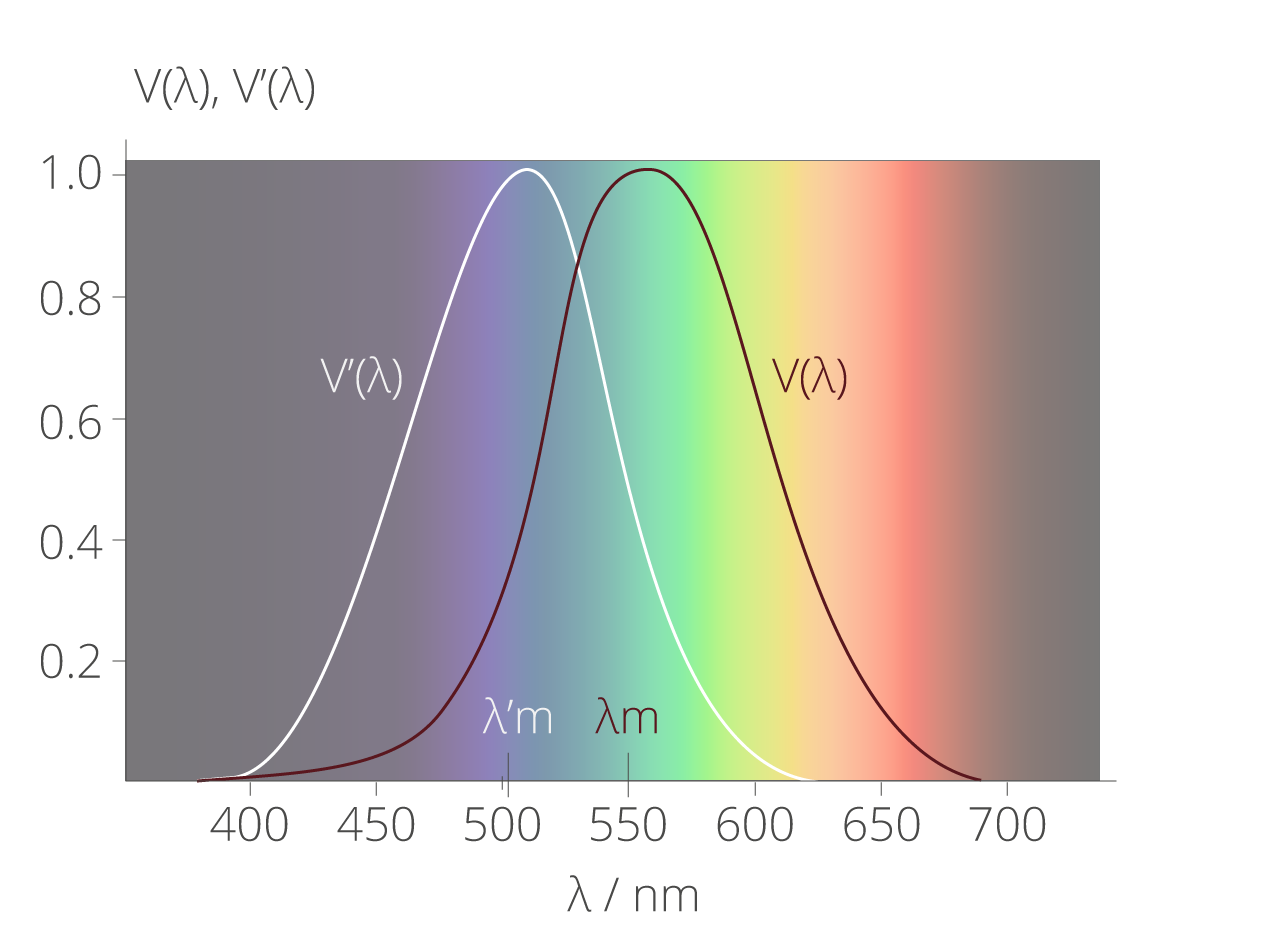
\includegraphics[width=0.7\textwidth]{bilder/augespek} 
% Bilddatei aus dem Unterverzeichnis bilder holen, skalieren auf 0.8*Satzspiegel
\caption {Zapfen und Stäbchen im Auge\protect\footnotemark}\label{b_augespek}
\end{figure}

\footnotetext{\url{https://www.gigahertz-optik.de/assets/Uploads/Abb.-II.13-neu-v03.png}}


\section{Sichtbares Spektrum} \label{sec_spektrum}

\section{Farbe} \label{sec_farbe}

\section{RGB Farbraum} \label{sec_rgb}

\section{CIE-XYZ Farbraum} \label{sec_xyz}

\section{CIE-LUV Farbraum} \label{sec_luv}

\section{CIE-LAB Farbraum} \label{sec_lab}

\chapter{Lichtechnische Parameter}

\section{Color Rendering Index (CRI)} \label{sec_cri}

Da der Farbort allein keine eindeutige Aussage über die Zusammensetzung des Spektrums zulässt, wurde 1931 von der CIE ein Testverfahren entwickelt, mit dem man die Farbwiedergabe (Color Rendering Index) einer Leuchte bestimmen kann. Dafür hat man acht Referenzfarben festgelegt. Bei einer CRI-Messung überprüft man also, wie gut eine Lichtquelle diese Körperfarben wiedergeben kann. Es wird dabei zwischen einem schwarzen Strahler(< 5000K) und Tageslicht(> 5000K) differenziert. Die gemessenen Unterschiede zu den Referenzfarben werden mit Werten von 0 bis 100 gewichtet($R_{1}$-$R_{8}$), wobei ein Wert von 100 aussagt, dass die Farbe bestmöglich wiedergegeben wird. Zuerst werden die einzelnen Indexwerte $R_{i}$ aus den Farbdifferenzen $\Delta E_{i}$ berechnet (Gleichung \ref{gl_cri1})\footnote{\cite{davis_ohno}}.

	\begin{equation}\label{gl_cri1}
		R_{i} = 100 - 4,6 \cdot \Delta E_{i}
	\end{equation}
Diese acht Werte werden schließlich arithmetisch gemittelt und es ergibt sich der Gesamtwert $R_{a}$ (Gleichung \ref{gl_cri2})\footnote{\cite{production partner}}.
	\begin{equation}\label{gl_cri2}
		R_{a} =\frac{1}{8} \sum_{i=1}^{8} R_{i}
	\end{equation}
In der DIN 6169 werden zur besseren Beurteilung der Farbwiedergabe die $R_{a}$-Werte in verschiedene Stufen unterteilt (Tabelle \ref{t_cri}).

	\begin{table}[htp] 
		\rowcolors{1}{}{lgray} 
		\centering
		\begin{tabular}{rlcc}  % Spalten nach Ausrichtung: l, c, r, p{breite} 
		\toprule
		\multicolumn{3}{c}{\large\sffamily Stufen des CRI}\\ 							
		\midrule
		1A & $R_{a} \geq 90$ & sehr hohe Anforderung\\ 
		1B & 90 > $R_{a} \geq 80$ & sehr hohe Anforderung\\
		2A & 80 > $R_{a} \geq 70$ & hohe Anforderung\\
		2B & 70 > $R_{a} \geq 60$ & hohe Anforderung\\
		3 & 60 > $R_{a} \geq 40$ & mittlere Anforderung\\
		4 & 40 > $R_{a} \geq 20$ & geringe Anforderung\\
		\bottomrule
		\end{tabular}
		\caption{$R_{a}$ eingeteilt in verschiedene Stufen\protect\footnotemark}	
		\label{t_cri}
	\end{table}
	\footnotetext{\cite[111]{hentschel}}

Ein hoher $R_{a}$-Wert beschreibt aber nur bedingt die Farbwiedergabe einer Leuchte, da beispielsweise keine Angabe über die Sättigung der Farben gemacht wird. Außerdem sind die acht Referenzfarben nur Pastelltöne, weil der CRI damals für Glühlicht entwickelt wurde. Gesättigte Farben fließen nicht in die Bewertung mit ein.
Das wirkt sich auch auf die Vergleichbarkeit von Leuchten aus. Zwei Scheinwerfer mit dem selben $R_{a}$-Wert von 90 können sehr unterschiedliche Spektren haben und damit sehr unterschiedlich Farben darstellen, trotz gleichem Farbwiedergabeindex.
Außerdem kann man nur schwer eine Aussage darüber machen, ob sich eine Leuchte mit einem guten CRI für Personenbeleuchtung eignet, weil Rottöne und Hauttöne in diesem Bewertungsverfahren fehlen.\\\\
Leuchtstofflampen nutzten den CRI aus, indem durch gezielte schmalbandige Peaks im Spektrum die Referenzfarben getroffen werden. Auf diese Weise kann zwar ein hoher CRI-Werte erreicht werden, aber kein breitbandiges und ausgefülltes Lichtspektrum entstehen. Daher sah sich die CIE gezwungen den Farbwiedergabeindex zu erweitern. In dem neueren $R_{e}$-Wert gibt es nun auch gesättigte Farben und eine Hautfarbe wird miteinbezogen (Abb. \ref{b_cri}).

\begin{figure}[htp]     % h=here, t=top, b=bottom, p=page
\centering
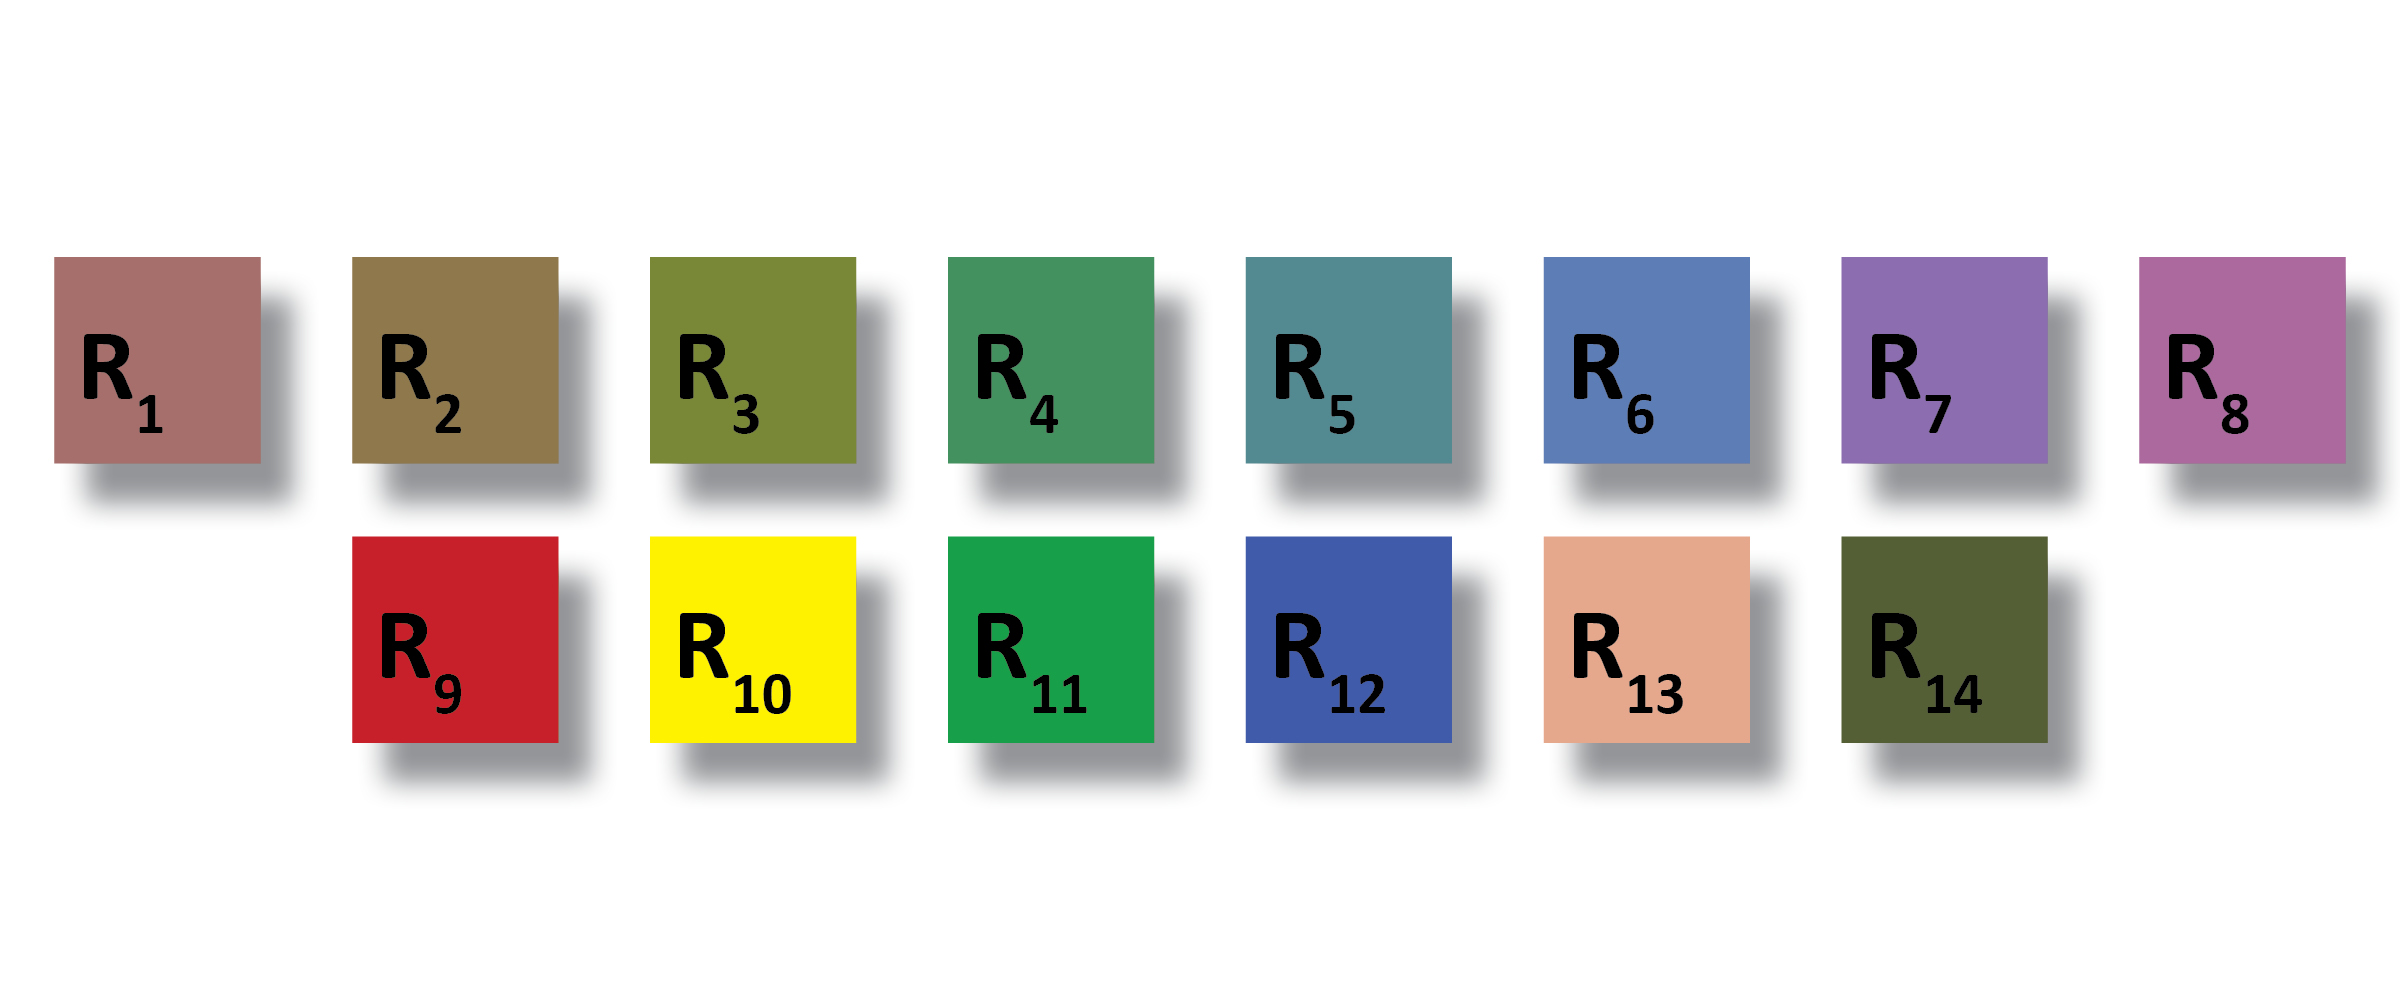
\includegraphics[width=0.8\textwidth]{bilder/cri} 
% Bilddatei aus dem Unterverzeichnis bilder holen, skalieren auf 0.8*Satzspiegel
\caption {Alle Referenzfarben des Farbwiedergabeindexes: $R_{1}$ Altrosa, $R_{2}$ Senfgelb, $R_{3}$ Gelbgrün, $R_{4}$ Hellgrün, $R_{5}$ Türkisblau, $R_{6}$ Himmelblau, $R_{7}$ Asterviolett, $R_{8}$ Fliederviolett, $R_{9}$ Rot gesättigt, $R_{10}$ Gelb gesättigt, $R_{11}$ Grün gesättigt, $R_{12}$ Blau gesättigt und $R_{13}$ Rosa (Hautfarbe), $R_{14}$ Blattgrün \protect\footnotemark}\label{b_cri}
\end{figure}

\footnotetext{\url{https://www.elementalled.com/wp/wp-content/uploads/2015/08/CRI_chart.jpg}}

Der $R_{e}$-Wert ist folglich schlechter als der $R_{a}$-Wert. Auch mit einem einzigen Rot- und Hautton ist der CRI zu wenig ausschlaggebend, um damit eine Leuchte für Personenbeleuchtung zu bewerten (Kap. \ref{sec_auge}). Zusätzlich entsteht bei LED-Leuchtmitteln ein ähnliches Problem, wie bei den Leuchstoffröhren. Man kann das Spektrum mit den Peaks gut auf die Referenzfarben ausrichten, ohne das Gesamte Spektrum abdecken zu müssen. Gerade bei LED-Leuchten kann dieses Verhalten des CRI ausgenutzt werden, um kritische Bereiche zu verschleiern. Zusätzlich wird dies durch die arithmetische Mittlung der Referenzfarbwerte begünstigt. Ein, zwei schlechtere Werte mindern den $R_{a}$-Wert nicht beträchtlich. Beispielsweise wird bei Weißen-LEDs  der fehlende Rotanteil nur am niedrigen $R_{9}$-Wert sichtbar, aber im im CRI-Wert sind diese Schwächen einer LED-Leuchte kaum erkennbar \footnote{\cite{davis_ohno}}. Der CRI kann daher eher als richtungsweisend betrachtet werden: Eine Leuchte mit guter Farbwiedergabe wird auch immer einen guten CRI-Wert haben. Zum Vergleich für Leuchten eignen sich andere Farbwiedergabewerte heutzutage besser \footnote{\cite{production partner}}.\\\\
Aus diesen Gründen und der Schlussfolgerung der CIE, \emph{\glqq dass die CRI-Methode generell nicht anwendbar ist, um eine Anzahl von Lichtquellen gemäß ihrer Farbwiedergabe einzuordnen, wenn weiße LEDs darunter sind\grqq}\footnote{\citep[VI]{CIE}}, wird sich diese Arbeit hauptsächlich auf andere Farbwiedergabewerte konzentrieren, den CRI aber mit aufführen, weil dieser in der Scheinwerfer- und Fernsehbranche (noch) einen hohen Stellenwert inne hat.

\section{Gamut Area Index (GAI)} \label{sec_gai}



\section{Color Quality Scale (CQS)} \label{sec_cqs}

Der Color Quality Scale, der von dem National Institute of Standards and Technology (NIST) erarbeitet wurde,orientiert sich an der Grundidee des CRI und versucht dessen Probleme anzugehen und ihn zu ersetzen. So gibt es fünfzehn voll saturierte Referenzfarben, die auch auf LED-Leuchten anwendbar sind. Über Skaleneffekte soll der CQS auch indirekt eine Aussage über die Farbwiedergabe von Pastelltönen ermöglichen. 

\begin{figure}[htp]     % h=here, t=top, b=bottom, p=page
\centering

\includegraphics[width=0.8\textwidth]{bilder/cqs} 
% Bilddatei aus dem Unterverzeichnis bilder holen, skalieren auf 0.8*Satzspiegel
\caption {Alle Referenzfarben des CQS mit voller Sättigung\protect\footnotemark}\label{b_cri}
\end{figure}

\footnotetext{\url{https://www.lemoledlight.com/wp-content/uploads/2016/04/LED-Lighting-CRI-5.jpg}}
Bei dem Farbvergleich des CRI wurden weniger Punkte für eine Farbe vergeben, wenn diese übersättigt wurde, also die Leuchte eine höhere Farbigkeit hatte als das Referenzlicht des CRI. Wenn beispielsweise eine Oberfläche eines Objekts beleuchtet wird, kann eine übersättigte Farbe jedoch hilfreich sein und ist daher nicht pauschal negativ einzuordnen. Daher wertet der CQS eine Übersättigung der Farbe nicht, nur eine Abweichung von Farbton oder Helligkeit wird bestraft. Außerdem errechnet sich der CQS aus dem quadratischen Mittel (root-means-square) der einzelnen Farben und es ist deutlicher erkennbarer, wenn einzelne Farbe schlechte Werte erzielen (Gleichung \ref{gl_cqs1})\footnote{\cite{davis_ohno}}.

\begin{equation}\label{gl_cqs1}
		\Delta E_{RMS} = \sqrt{\frac{1}{15} \sum_{i=1}^{15} \Delta E_{i} ^{2}} 
\end{equation}

Schließlich wird beim CQS verhindert, dass negative Werte vorkommen, die beim CRI stets schwierig zu interpretieren sind. 



\section{Television Lighting Consistency Index (TLCI)} \label{sec_tlci}



\section{IES Method for Evaluating Light Source Color Rendition (TM-30-15)} \label{sec_tm30}

\chapter{Leuchtmittel}

\section{Glühlampe} \label{sec_glühlampe}

\section{Halogenglühlampe} \label{sec_halogenglühlampe}

\section{Entladungslampen} \label{sec_entladungslampe}

\section{LEDs} \label{sec_led}

\chapter{Vormessungen}

\section{Ziel}

\section{Aufbau}

\section{Fazit aus der Vormessung}

\chapter{Hauptmessung}

\section{Messaufbau}

\chapter{Messergebnisse}

\section{Unterkapitel mit Mathematik, Bildern und Querverweisen}

\chapter{Umfrage}

\section{Unterkapitel mit Mathematik, Bildern und Querverweisen}

\chapter{Umfrageergebnisse}

\section{Unterkapitel mit Mathematik, Bildern und Querverweisen}

\chapter{Auswertung aller Ergebnisse}

\section{Unterkapitel mit Mathematik, Bildern und Querverweisen}

\chapter{Fazit}

\section{Unterkapitel mit Mathematik, Bildern und Querverweisen}





%--------------------- VERZEICHNISSE ----------------

\listoffigures % Abbildungsverzeichnis erzeugen
\listoftables % Tabellenverzeichnis erzeugen

%--------------------- LITERATURLISTE ---------------
% Die Einträge sollen alphabetisch sortiert sein.

\begin{thebibliography}{}

% Formatierung für Internetquelle
% Grundregel: Name, Vorname (falls vorhanden), VÖ-Jahr (falls vorhanden), Titel in Anführungszeichen, URL, Datum des letzten Aufrufs
% zur Formatierung der URL unbedingt den url-Befehl benutzen!!!


\bibitem[Commission Internationale de l'Eclairage(2007)]{CIE}
Commission Internationale de l'Eclairage:
\emph{\glqq Technical Report 177:2007 : Color Rendering of White LED Light Sources\grqq}
\url{https://de.scribd.com/document/125319182/CIE-177-2007}, 2007, letzter Zugriff 20.06.2018

\bibitem[Davis \& Ohno(2006)]{davis_ohno}
Davis, Wendy L. \& Ohno, Yoshihiro:
\emph{\glqq Development of a Color Quality Scale\grqq}
\url{http://citeseerx.ist.psu.edu/viewdoc/download?doi=10.1.1.568.8399&rep=rep1&type=pdf}, 08.02.2006, letzter Zugriff 20.06.2018

\bibitem[DocCheck Flexikon(2014)]{doccheck sko}
DocCheck Flexikon:
\emph{\glqq Skotopisches Sehen\grqq}
\url{http://flexikon.doccheck.com/de/Skotopisches_Sehen}, 24.01.2014, letzter Zugriff 18.06.2018

\bibitem[DocCheck Flexikon(2014)]{doccheck pho}
DocCheck Flexikon:
\emph{\glqq Photopisches Sehen\grqq}
\url{http://flexikon.doccheck.com/de/Photopisches_Sehen}, 10.05.2016, letzter Zugriff 18.06.2018

\bibitem[Production Partner(2018)]{production partner}
Production Partner:
\emph{\glqq Farbwiedergabe: TM-30-15, CRI und Co.\grqq}
\url{https://www.production-partner.de/basics/farbwiedergabe-tm-30-15-cri-und-co/}, 22.02.2018, letzter Zugriff 20.06.2018


\bibitem[Gigahertz-Optik(2012)]{Gigahertz}
Gigahertz-Optik:
\emph{\glqq Grundladen der Lichtmesstechnik\grqq}
\url{https://www.gigahertz-optik.de/de-de/grundlagen-lichtmesstechnik/}, letzter Zugriff 20.06.2018


% Formatierung für Aufsatz / Paper: Titel in Anführungszeichen, Zeitschriftentitel kursiv
\bibitem[Dooley \& Streicher(1982)]{dooley_streicher} 
Dooley, Wesley L.  \& Streicher, Ronald D.:
\glqq M--S Stereo: A Powerful Technique for Working in Stereo\grqq, 
\emph{Journ. Audio Engineering Society} vol. 30 (10), 1982

% Formatierung für Fachbuch, Diplomarbeit o.Ä.: Titel kursiv

\bibitem[Hentschel(1993)]{hentschel}
Hentschel, Hans-Jürgen: 
\emph{Licht und Beleuchtung Theorie und Praxis der Lichttechnik}, 4. Aufl., Hüthig 1994

% Formatierung für Fachbuch mit Herausgeber und mehreren Autoren
\bibitem[Spehr(2009)]{spehr}
Spehr, Georg (Hrsg.): 
\emph{Funktionale Klänge}, transcript 2009

\bibitem[Greule(2014)]{greule}
Greule, Roland (Autor):
\emph{Licht und Beleuchtung im Medienbereich}, Hanser 2015 


% Formatierung für ein einzelnes Kapitel eines speziellen Autors aus einem Fachbuch mit mehreren Autoren
\bibitem[Sowodniok(2009)]{sowodniok}
Sowodniok, Ulrike: 
\glqq Funktionaler Stimmklang -- Ein Prozess mit Nachhalligkeit\grqq, 
in: Spehr, Georg (Hrsg.): \emph{Funktionale Klänge}, transcript 2009




% Formatierung für Aufsatz / Paper: Titel in Anführungszeichen, Zeitschriftentitel kursiv
\bibitem[Stephenson(1990)]{stephenson}
Stephenson, Uwe: 
\glqq Comparison of the Mirror Image Source Method and the Sound Particle Simulation Method\grqq, 
\emph{Applied Acoustics} vol. 29, 1990


\end{thebibliography}

%--------------------- EIGENSTÄNDIGKEITSERKLÄRUNG ---------------
\clearpage\thispagestyle{empty}
\eigen  % im header definiert
%--------------------------------------- ENDE ------------------------------------
\end{document}
%%%%%%%%%%%%%%%%%%%%%%%%%%%%%%%%%%%%











